\documentclass[a4paper,12pt]{article}
\usepackage[margin=2.5cm,letterpaper]{geometry}
\usepackage{authblk}
\usepackage{setspace}
\usepackage{subfig}
\usepackage{amsmath}
\usepackage{amsfonts}
\usepackage{amssymb}
\usepackage{caption}
\usepackage{graphicx}

\usepackage[super,comma,sort&compress]{natbib} % enhances bibtex citations
%\usepackage{hypernat}
\usepackage[english]{babel}
\usepackage[T1]{fontenc} %Useful for file names with underscores in them
\usepackage{float}
\usepackage{grffile}
\newcommand{\hilight}[1]{\colorbox{yellow}{#1}} %To highlight text
\renewcommand{\thefootnote}{\alph{footnote}} %For footnotes
%\usepackage{hyperref}


\title{The effect of gravity on the stability of an evaporating dichloromethane liquid film}

\author[1]{Aneet D. Narendranath}
\author[2]{James C. Hermanson}
\author[3]{Robert W. Kolkka}
\author[3]{Allan A. Struthers}
\author[1]{Jeffrey S. Allen \thanks{jstallen@mtu.edu}}
\affil[1]{Mechanical Engineering-Engineering Mechanics, Michigan Technological University, Houghton, MI}
\affil[2]{Aeronautics \& Astronautics, University of Washington, Seattle, WA}
\affil[3]{Mathematical Sciences, Michigan Technological University, Houghton, MI}


\begin{document}
\maketitle 

\begin{abstract}
\noindent Zero gravity evaporation of a Dicholoromethane (DCM) liquid film is explored. The resulting film dynamics are presented and a criterion for stable films is described based on the long wave theory. It is concluded that films subject to long wave instabilities shows the appearance of the mode of maximum growth rate at rupture, irrespective of the initial condition or domain size conditions. Films stable in Earth's gravity are destabilized in zero gravity.

\end{abstract}



\section{Impact of liquid films}
%\doublespacing
Liquid films and coatings find applications in several areas of technology, physics and biology as their flows occur over a large range of length scales \citep{Craster2009a}. Coatings receive widespread attention in several industries. They are used as lubricants, paint for rust prevention and aesthetics in architecture, in time release capsules and tablets in the medical industry, the paper and pulp industry and the microelectronics fabrication industry. Liquid films find applications in the food processing industry \citep{Pehlivan2012a, Moresi1988a}, cooling of server towers (which was a \$36 Billion industry in 2007) \citep{Agostini2007a, Darabi2003a, Marcinichen2010a} and for improved oil recovery from petroleum reservoirs \citep{Schramm1992a, Bergeron1993a}. A report from the Brookhaven National Laboratory estimated that in excess of \$100 billion per year, is spent on the prevention and remediation of rust damage \citep{Cheremisinoff2003a}.\\

One of the earliest commentaries to study liquid films was by Rayleigh\citep{Rayleigh1916a} wherein he described convective cells in \emph{spermacetti} heated from below and the corresponding wavelength associated with this convection pattern. It was suggested by Rayleigh that this convection was driven by surface tension. This was corrected later, notably, by Pearson \citep{Pearson1958a} who suggested that given the rigid-rigid boundary conditions used by Rayleigh could not have allowed for surface tension gradients to drive the convection. Rayleigh's observations were deemed to be due to buoyancy effects. Pearson conducted an examination of liquid films heated from below and subject to rigid-free boundary conditions at the bottom and top respectively to uncover surface tension driven convection. These convection cells were thereafter referred to as Pearon cells. Scriven and Sterling provided numerical methodology for a similar situation as that which gave rise to the ``Pearson cells'.  In their case, the surface was assumed to be infinitesimally deformed via long waves. Scriven and Sterling's work paved the way for the long wave theory. The long wave theory (LWT) was further explored shortly after by Benney \citep{Benny1966a, Benny1966b} to describe the interactions of long wavelength disturbances in falling films.\\

The study of long wave interactions on the surface of liquid films gained significant impetus when Davis et al. \citep{WandD} and later Burelbach et al.\citep{Burelbach} developed a non-linear evolution equation to describe the film dynamics of an evaporating liquid film. The essense of the Navier-Stokes' equations was rolled into this evolution equation. This equation has been used since for a variety of problems concerning liquid films that could be categorized under problems of the lubrication approximation type/long wavelength phenomena.\\

This theoretical treatment can be traced far back to Benney \citep{Benny1966b}. The evolution equation, as a result of applying the LWT to the Navier Stokes' equations has been successfully used to analyse liquid film dynamics and several instances can be found in literature \citep{Krishnamoorthy1995a, Vanhook1997a, Oron1997a, Oron2000b}.\\

The general trend in literature since the development of the evolution equation has been the simulation of non-evaporating liquid films via LWT/evolution equation \citep{Krishnamoorthy1995a, Vanhook1997a, Oron2000b, Sultan2005a, Dietzel2009a}. The stability of evaporating liquid films were analysed in two-dimensional space by Burelbach \cite{Burelbach} and in three-dimensional space by Oron \citep{Oron2000b, Oron2000c}. The former lacked three-dimensional simulations while the latter did not attempt a solution to the complete evolution equation for evaporating liquid films and neglected  mass loss and destabilization by vapor recoil in favor of disjoining pressures.\\

There is a paucity of research on zero gravity film dynamics. Pradhan and Samal \citep{Pradhan1987a} and Straughan \citep{Straughan1989a} performed some normal mode analysis on the full Navier Stokes' equations in zero gravity.  Studying zero gravity film dynamics is important as zero gravity environments help isolate a system from terrestrial gravity effects. Understanding the instabilities that affect fluids and liquid films in zero gravity is important as capillary forces could become significant and could govern the behavior of the liquid system. For instance, propulsion systems or water recovery systems that employ or recover liquids would behave differently in low gravity as compared to an Earth like gravity field. Evaporation in such systems may not allow the liquid and the gas phases to separate into two distinct components due to a lack of buoyancy \citep{Ostrach1982a}.\\

In this article, a modified evolution equation describing evaporating liquid film dynamics is solved numerically as an initial value problem to describe a slowly evaporating Dicholoromethane liquid film in zero gravity and Earth's gravity. The importance of gravity in dictating film dynamics is studied. \\


\section{Evolution equation describing dynamics of an evaporating liquid film}

The evolution equation derived from the LWT, describing an evaporating Newtonian liquid film is given by equation \ref{evolution1}. The non-dimensional parameters, viz., $E, S, Ga, E, D, K, M, Pr, Ra$  are expressed in table \ref{tab:nomenclature}.


%are the evaporation numer (ratio of viscous time scale to evaporation time scale), non-dimensional measure of surface tension, Marangoni number and the degree of non-equilibrium at the interface, respectively. For detailed definitions, the reader is directed to Burelbach et al. \citep{Burelbach}. $Ga$ is the Galileo number which describes the stabilizing effect of gravity on the interface and is defined as $g h_0^3/\nu^2$ where $h_0$ is the initial film thickness, $\nu$ is the kinematic viscosity and $g$ is the acceleration due to gravity. Pr is the Prandtl number defined as the ratio of kinematic viscosity to thermal diffusivity, $\nu/\kappa$. $Ra$ is the Rayleigh number defined as $g \beta \Delta T h_0^3/ \nu\kappa$. This was introduced by us in the evolution equation \ref{evolution1} by including the Boussinesq approximation in the momentum equation. The Marangoni number is defined as $M = \frac{\sigma_T \Delta T h_0}{\rho \nu \kappa}$. The evaporation number is defined as $E=k \Delta T/\rho \nu \L$ where $L$ is the latent heat for the liquid. $E$ is a ratio of viscous time scale to the evaporation time scale and for slow evaporation, $E$. The non-dimensional surface tension is defined as $S=\sigma h_0/\rho \nu^2$. The measure of non-equilibrium at the interface is defined as $K = \frac{k T_{sat}^{3/2}}{\alpha h_0 \rho^v L^2} \left(\frac{2 \pi R_g}{M_w}\right)^{1/2}$. Here, $\alpha$ is the accommodation coefficient, $R_g$ is the universal gas constant and $M_w$ is the molecular weight of the liquid.
% 
% \begin{align} \label{evolution1}
%  h_T + \frac{E}{(h + K)} + S(h^3h_{XXX})_X \nonumber \\
% - \frac{Ga}{3}(h^3h_X)_X + E^2D^{-1}\left[ \frac{h^3 h_X}{(h + K)^3}\right]_X + \nonumber \\
%  KMPr^{-1} \left[ \frac{h^2h_X}{(h + K)^2}\right]_X + \nonumber \\ 
% \frac{5 Ra}{48 \text{Pr}} \left[\frac{K^2}{(h+K)^2}h^4 h_X + h^4 h_X \right] &= 0
% \end{align}

\begin{align} \label{evolution1}
 h_T + S \nabla \cdot (h^3 \nabla \nabla^2 h) - \frac{Ga}{3} \nabla \cdot (h^3 \nabla h)  \nonumber \\
+ \nabla \cdot \left[ \left( E^2 D^{-1} \frac{h^3}{(h + K)^3} + KM\text{Pr}^{-1} \frac{h^2}{(h + K)^2} \right) \nabla h \right] \nonumber \\
 \frac{5 Ra}{48 \text{Pr}} \left[ \frac{K^2}{(h + K)^2}h^4 + h^4\right] \nabla h = 0 
\end{align}



Using $S$ to scale the various terms in the evolution equation and using the linear stability theory, the wavenumber corresponding to the fastest growing wavenumber is derived and presented in equation \ref{wavenumber_eqn}.  The fastest growing wavelength is merely $2\pi/q_\text{max}$ where $2\pi$ is the length of the domain. 


% \begin{align} \label{wavenumber_eqn_}
%  q_\text{max} = \left[ \frac{-Bo \overbar{h}^3 + \delta \overbar{h}^3 (\overbar{h} + K)^{-3} +m \overbar{h}^2 ( \overbar{h} + K)^{-2}) + R \{\frac{K}{(h + K)^2} - 1\} \overbar{h}^4}{2 \overbar{h}^3 }  \right]^{\frac{1}{2}} \nonumber
% \end{align}

% \begin{align} \label{wavenumber_eqn}
%  q_\text{max} = \left [ \frac{-Bo + \delta (h + K)^{-3} + \frac{m}{h}(h + K)^{-2} + R h \{ \frac{K}{(h + K)^{2}} - 1 \}}{2} \right]^{1/2} \nonumber \\
% \lambda_\text{max} = \frac{2 \pi}{q_\text{max}}
% \end{align}

\begin{align} \label{wavenumber_eqn}
 \text{q}_\text{max} = \sqrt{\frac{-Bo}{2} + \frac{\delta}{(h + K)^3} + \frac{m}{2 h (h + K)^2}} 
% \lambda_\text{max} = \frac{2 \pi}{\text{q}_\text{max}}
\end{align}

Here $Bo = G/S, \delta = E^2/DS$, $m = MK/\text{Pr}S$ and $R = 5 Ra/48\text{Pr}S$ are respectively the Bond number, evaporative effects of mass loss and vapor recoil, thermocapillarity number. 

There are several advantages to scaling the evolution equation with the surface tension number, $S$. The evolution equation is generally scaled with a combination of $Ga$ and $S$. However, involving the Galileo number, $Ga$, in the scaling leads to undesirable divide by zero errors when exploring film dynamics in zero gravity environments. The scaling method used here to arrive at the fastest growing wavelength allows for zero gravity film dynamics to be explored. 
%In our linear stability analysis we perturbed the film with a time varying disturbance of the form $h = \overbar{h(T) + H(t)e^{i \text{q} X}}$ where q is the disturbance wavenumber and X is the longitudinal dimension scaled by the mean initial film thickness ($X = x/h_0$). 

%\subsection{Different versions of the evolution equation in literature}
%When literature is perused, it is natural to come across two different versions of the evolution equation and the resulting equation for the fastest growing wavelength. Close examination reveals that the difference lies in the definition of $m$. In case an evaporating liquid film is under investigation, at the interface, the constitutive relationship of Wayner/Schrage \citep{Wayner1976a} is used to link the fluid and vapor regions through an evaporative mass flux. This results in $m$ being defined as $M K /\text{Pr}$. In case a non-evaporating liquid film is under investigation, the liquid and vapor phases are linked via a Robin boundary condition for the equality of conduction and convection at the interface. This results in a Biot number, $Bi$ and $m$ is defined as $M \text{Bi}/\text{Pr}S$. As our evolution equation simulates evaporating liquid films, we define $m$ as $M K /\text{Pr}$. 

%If we so please, a combined form of $m$ could be used for a ``global'' evolution equation as depicted in equation \ref{mequation}

%\begin{align} \label{mequation}
% m = \frac{M \eta}{\text{Pr}S}
%\end{align}
%The value of $\eta$ could be Bi or $K$ depending on the situation. For a non-evaporating liquid film, if thermocapillarity were to be captured, $\eta = \text{Bi}$. For an evaporating liquid film, if thermocapillarity were to be captured, $\eta=K$.


\subsection{Validation}

%The ``mathematical fluid'' are fluid properties most often used in literature \citep{Krishnamoorthy1995a, Oron2000b}. The ``mathematical fluid'' represents fluid properties leading to a maximum growth rate of thermocapillary structures. The closest physical fluid mirroring the properties of this mathematical fluid is perhaps a low centistoke Silicone oil \citep{Vanhook1997a}.

% In equation \ref{wavenumber_eqn}, $Bo = Ga/S, \delta = E^2/DS, m = M K/\text{Pr}S, R = (5/48) (Ra/\text{Pr}S)$ where $D$ is the vapor to liquid 
% density ratio $\rho_v/\rho_l$. For the one sided model in equation \ref{evolution1}, $D \textless \textless 1$. 

The evolution equation has been verified and validated against literature \citep{Krishnamoorthy1995a, Oron2000b} by comparing film dynamics for non-evaporating cases. We use slowly evaporating films ($E=0.0001$) whose fastest growing wavelength are not far removed from non-evaporating liquid films. The fastest growing wavelength for various non-evaporating, evaporating situations is tabulated in table \ref{tab1}. This serves as a comparison with literature \citep{Krishnamoorthy1995a, Oron2000b} and validation of our expression (termed ``MTU/UW'') for the fastest growing wavelength as in equation \ref{wavenumber_eqn}.

%The evolution equation \ref{equation1}, was solved as an initial value problem with periodic boundary conditions with the LSODE solver in the Mathematica environment. We compared our numerical results with those of \citet{Oron2000b, Krishnamoorthy1995a} and have concluded that our code produces results within $5\%$ of literature.
Table \ref{tab1} shows a comparison with the fastest growing wavelength as calculated by Oron \citep{Oron2000b}.  The first row is a validation of our expression for the fastest growing wavelength, equation \ref{wavenumber_eqn}. The second and third rows of table \ref{tab1} show the influence of increasing the number of mechanisms (viz., lack of gravity, evaporative mass flux, non-equilibrium at the interface) that affect the dynamics of a liquid film.

It is observed from table \ref{tab1} that for a slowly evaporating liquid film with an $E=0.0001$, the fastest growing wavelength is not affected strongly by evaporative mass flux and vapor recoil when the $Ga=0.333$. However, it is noticed from table \ref{tab1} that in the case of zero gravity evaporation, the film is susceptible to shorter wavelengths for slow evaporation rates.

The evolution equation \ref{evolution1}, was solved as an initial value problem with periodic boundary conditions with the LSODE solver \citep{Hindmarsh1987a} in the Mathematica environment \citep{Struthers2010a}. We compared our numerical results with those of Oron \citep{Oron2000b} and  Krishnamoorthy\citep{Krishnamoorthy1995a} and have concluded that our code produces results within $5\%$ of literature. We used film profile plots in conjunction with discrete Fourier transform plots (with their DC component zeroed) to analyse the film structure and the frequency trends of evaporating DCM liquid films.


% \begin{table}[h]
% \caption{Comparison of fastest growing wavelength, $\lambda_\text{max}$. $\text{Pr}=7.02$ as per Oron et al. \citep{Oron2000b}, Krishnamoorthy et al. \citep{Krishnamoorthy1995a}. The first row shows a comparison/validation of the fastest growing wavelength as derived by us with equation with that of \citet{Oron2000b}}
% \label{tab1}
% \begin{center}
% \hline
% \begin{tabular}{|p{4cm}|p{3cm}|p{3cm}|}
% Case & Literature \citep{Oron2000b,Krishnamoorthy1995a} & MTU/UW\\
% \hline
% $S=100, Ga=0.333, M=35.1$ & 93.78 & 93.78 (validation)\\
% $S=100, Ga=0.0, M=35.1$ & -- & 92.322\\
% $E=0.0001, Ga=0.0, M=35.1, K=1.0$ & -- & 79.1712 \\
% \hline
% \end{tabular}
% \end{center}
% \end{table}


\section{Definition of rupture}
It has been propounded that when a film ruptures on a substrate, an adsorbed layer is left behind whose depletion is a function of the wetting nature\citep{Oron2001a} of the film on this substrate. Rupture is defined as that juncture in time when the the film recedes from the surface depending on the surface wetting characteristics. Disjoining pressure terms would need to be included in the evolution equation, \ref{evolution1} to study film rupture via dewetting on the surface.

We do not include the effect of wetting via Van der Waal's forces in the evolution equation. From hereon, we define rupture as that juncture in the computation when the effect of various non-linear terms in the evolution equation is to induce numerical stiffness at small film thicknesses. In our simulation cases, rupture occurs when the film thickness reaches about 3-4\% of the initial film thickness. Physically, this rupture thickness translates to about $250 \mu m$ for the dichloromethane film we simulate. From the discrete Fourier transform (DFT) plots (eg. figure \ref{fig_ic_effect}), at rupture, the film profile shows the appearance of high frequency Fourier modes. The utility of the DFT plots is enabling the realization that as the film progresses toward rupture, higher frequencies appear. The fastest growing wavelength is the dominant mode. A cascade of higher frequencies is seen as gray spots. The DFT plots show all those frequencies that account for $10\%$ or more of the total energy at that stage in time.

\section{Dichloromethane liquid film evaporating in zero gravity}

Two different initial conditions are used to perturb a DCM film evaporating in zero gravity. Figure \ref{fig_ic} a smooth cosine initial condition and it's discrete Fourier transform (DFT) frequency distribution is compared against a uniform random distribution. The smooth initial condition is generally used in literature.

 The evolution equation \ref{evolution1} is solved to simulate a 2.35mm thick Dichloromethane liquid film which is slowly evaporating. The non dimensional parameters for the Dichloromethane liquid film are compared with that of the mathematical fluid in table \ref{dcm_math_comparison}. The film is placed in a square domain whose side length is equal to about $5$ inches ($\lambda_\text{max} \approx 5$ inches for a $2.35$ mm DCM film). When the film is perturbed by a smooth initial condition or a uniform random initial condition the film ruptures via long wave type/thermocapillary driven structures. The end result in figure \ref{fig_ic} shows a cascade of Fourier modes in zero gravity. The dominant mode in the DFT plot is that which corresponds to the fastest growing wavelength, with the maximum growth rate.

However, when the DCM evaporates in Earth's gravity, the film is resistant to long wave type instabilities as seen by the blank DFT plot in figure \ref{fig_ic_effect} \subref{fig:2a}. Hence a DCM film that is resistant to thermocapillary rupture in Earth's gravitational field is destabilized in zero gravity and is driven to rupture. Another interesting observation is that in Earth's gravity, the complete depletion of the liquid film takes place in about 1 minute. However, in a zero gravity environment, the film ruptures in around 4 seconds.


% \begin{table}
% \begin{center}
% \begin{tabular}{|l|l|l|l|} 
% \hline
%  & $g=9.81 m/s^2$ & $g=0 m/s^2$ & Math fluid\\
% \hline
% G & $4.11 \times 10^6$ & 0 & 0 / 0.333\\
% S & $143 \times 10^3$ & $143 \times 10^3$ & 100\\
% Bo & $28.74$ & $0$ & $0.0333$ \\
% M & $122 \times 10^3$ & $122 \times 10^3$ & 35.1\\
% Pr & $3.9$ & $3.9$ & 7.02\\
% m & $0.218$ & $0.218$ & $0.05$ \\
% $\epsilon$ & $6.01 \times 10^-8$ & $6.01 \times 10^-8$ & 0\\
% $\delta$ & $5.19 \times 10^-7$ & $5.19 \times 10^-7$ & 0 \\
% \hline
% \end{tabular}
% \end{center}
% \caption{Comparison of non-dimensional numbers}
% \label{dcm_math_comparison}
% \end{table}

%The fluid parameters for DCM are compared with those of the mathematical fluid in table \ref{dcm_math_comparison}. Comparison of film dynamics of an evaporating 2.35mm Dichloromethane liquid film from figures \ref{fig_eg} and \ref{fig_zg} reveal interesting characteristics. In Earth's gravity (fig \ref{fig_eg}), the Bond number, $Bo$, is considerably stronger than the thermocapillarity numer, $m$. When this is the case all long wave modes are stabilized by surface tension and gravity and the only significant observation is the finite time evaporation of the film. In zero gravity (fig \ref{fig_zg}), the Bond number is zero. In other words, the film would be destabilized due to thermocapillarity and rupture would occur via long wave modes/thermocapillary fingers. 
%The growth rate of instabilities calculated from the equation for growth rate shows, concurrent to the observation, a negative growth rate or a damping effect.

% However, when the effect of gravity is turned off by setting $g=0.0 m/s^2$ and hence $Ga=0.0$, we nullify the stabilizing effect of the Bond number term. Thermocapillarity causes vulnerability to long wave destabilization. The film eventually ruptures in about 4 seconds (physical time). Thermocapillary fingers are seen at rupture.


%   \begin{figure} 
%    \centering
%     \subfloat{\includegraphics[width=0.45\linewidth]{ic}\label{fig:1a}} 
%     \subfloat{\includegraphics[width=0.45\linewidth]{grup}\label{fig:1b}} 
%     \subfloat{\includegraphics[width=0.45\linewidth]{ic_dft}\label{fig:1c}}
%     \subfloat{\includegraphics[width=0.45\linewidth]{grup_dft}\label{fig:1d}}
%    \caption{2.35 millimeter DCM film evaporating in Earth's gravitational field. Film is depleted in 1 minute.}
%    \label{fig_zg}
%   \end{figure}



%  \begin{figure} 
%    \centering
%     \subfloat{\includegraphics[width=0.45\linewidth]{ic}\label{fig:2a}} 
%     \subfloat{\includegraphics[width=0.45\linewidth]{zg_rup}\label{fig:2b}} 
%     \subfloat{\includegraphics[width=0.45\linewidth]{ic_dft}\label{fig:2c}}
%     \subfloat{\includegraphics[width=0.45\linewidth]{zg_rup_dft}\label{fig:2d}}
%    \caption{2.35 millimeter DCM film evaporating in zero gravity. Film is depleted in 4 seconds. Thermocapillary fingers/long wave structures appear at rupture.}
%    \label{fig_eg}
%   \end{figure}




%\subsection{Summary: Evaporating DCM film in Earth gravity and zero gravity \label{sec1_conclusions}}

%\begin{enumerate}
% \item The 2.35mm Dichloromethane liquid film evaporates swiftly and with the presence of long wave instabilities in zero gravity.
% \item In Earth's gravity, the long wave modes are damped out by a combined stabilizing effect of gravity and surface tension.
% \item Gravity stabiliziation has technological implications: Long wave thermocapillary instabilities and concurrent rupture occur for a liquid film in zero gravity, although this film may be thick enough to resist long wave modes in regular gravity.
%\end{enumerate}


%\section{Evaporating DCM film with noisy uniform distribution as the initial condition}

%A noisy initial condition from a uniform distribution is used as aperturbation for the evaporating Dichloromethane film. The choice of this noisy initial condition reflects the need to model the effect of realistic perturbations on film dynamics. This noisy initial condition was applied to an evaporating DCM film, $2.35$ millimeter thick, evaporating in zero gravity. Two different domain sizes are used: one is a square domain with it's side-length a whole number multiple or a non-whole number multiple of the fastest growing wavelength. The other was a rectangular domain with length and breadth being non-whole number multiples of the fastest growing wavelength. The film dynamics are plotted in figures \ref{random_1},\ref{random_1_repeat}, \ref{rndm2}.


%\subsection{Square whole number domain}


%\subsection{Square non-whole number domain}

The domain size is now changed for this DCM film evaporating in zero gravity. We use a square domain with $L=2.238 \lambda_\text{max}$ and a rectangular domain with $L_x=2.238 \lambda_\text{max}, L_y=1.641\lambda_\text{max}$. When the film is perturbed with a uniform random initial condition a cascade of frequencies with the fastest growing wavelength as the dominant mode emerges as seen in figure \ref{fig_domain_size_effect}.

%A non-whole number domain is one in which the square side dimension is a non-whole number of the fastest growing wavelength for a slowly evaporating DCM film in zero gravity. The side length is $L_x = 2.238 \times \lambda_\text{max}$. A uniform random initial condition perturbs the DCM film and it is allowed to evaporate. The initial perturbation allows for the growth of thermocapillary finger structures. The DFT plot shows that the dominant mode at rupture is that of the fastest growing wavelength. There is a directional preference of the dominant mode for this non-whole number domain.

%To rule out any ``weird effects" (don't know what to call them yet), this case with the uniform random disturbance is run again. The rupture structure is not identical for the second run but the frequency trends match with a directional preferences for the dominant mode. This is seen in figure \ref{random_1}, \ref{random_1_repeat}

%\subsection{Rectangular non-whole number domain}

%A non-whole number rectangular domain is used next with the length and width of the rectangle respectively are $L_x = 2.238 \times \lambda_\text{max}$ and $L_y=1.641 \times \lambda_\text{max}$. The uniform random initial perturbation is allowed to grow via thermocapillarity as the film evaporates. The dominant mode at rupture is the fastest growing wavelength. There is a cascade of frequencies that is observed in figure \ref{rndm2}.

%   \begin{figure} 
%    \centering
%     \subfloat{\includegraphics[width=0.45\linewidth]{/home/dnaneet/Research/Dissertation/wigner/ic/random/DCM/dftdata/dcm_2350micrometer_profile_0}\label{fig:1a}} 
%     \subfloat{\includegraphics[width=0.45\linewidth]{/home/dnaneet/Research/Dissertation/wigner/ic/random/DCM/dftdata/dcm_2350micrometer_profile_Rup}\label{fig:1b}} \\
%     \subfloat{\includegraphics[width=0.45\linewidth]{/home/dnaneet/Research/Dissertation/wigner/ic/random/DCM/dftdata/dcm_2350micrometer_dft_0_corner}\label{fig:1c}}
%     \subfloat{\includegraphics[width=0.45\linewidth]{/home/dnaneet/Research/Dissertation/wigner/ic/random/DCM/dftdata/dcm_2350micrometer_dft_corner_Rup}\label{fig:1d}}
%    \caption{2.35 millimeter DCM film evaporating in zero gravity, subject to a uniform random initial condition. Film is depleted in 4 seconds. The fastest growing wavelength appears at rupture.}
%    \label{random_1}
%   \end{figure}


%   \begin{figure} 
%    \centering
%     \subfloat{\includegraphics[width=0.45\linewidth]{/home/dnaneet/Research/Dissertation/wigner/ic/random/DCM/dftdata/dcm_2350micrometer_nonwhole_lx_ly_profile_0}\label{fig:1a}} 
%     \subfloat{\includegraphics[width=0.45\linewidth]{/home/dnaneet/Research/Dissertation/wigner/ic/random/DCM/dftdata/dcm_2350micrometer_nonwhole_lx_ly_profile_Rup}\label{fig:1b}} \\
%     \subfloat{\includegraphics[width=0.45\linewidth]{/home/dnaneet/Research/Dissertation/wigner/ic/random/DCM/dftdata/dcm_2350micrometer_nonwhole_lx_ly_dft_0_corner}\label{fig:1c}}
%     \subfloat{\includegraphics[width=0.45\linewidth] {/home/dnaneet/Research/Dissertation/wigner/ic/random/DCM/dftdata/dcm_2350micrometer_nonwhole_lx_ly_dft_corner_Rup}\label{fig:1d}}
%    \caption{Evaporating Dichloromethane (DCM) film evolving after a uniform rando initial condition is imposed in zero gravity. The initial film thickness is $2.35 mm$. The domain is rectangular with length and breadth respectively equal to $2.238 \lambda_\text{max}$ and $1.641 \lambda_\text{max}$. Cascade of superharmonics appears in the longer dimension. The fastest growing wavelength holds most of the energy at rupture. Film ruptures in 4 seconds.}
%    \label{rndm2}
%   \end{figure}


%\subsection{Summary: Effect of noisy random initial condition on evaporating DCM in zero gravity}
%As observed in figures \ref{random_1},\ref{random_1_repeat}, \ref{rndm2}, imposing a realistic noisy initial condition resulted in the appearance of the fastest growing wavelength as the dominant mode at rupture. The effect that the domain shape and size had is the introduction of secondary structures and directional preference for the secondary structures. The secondary structures are seen as a cascade of superharmonics in the DFT plots at rupture.

\section{Criterion for film thickness for long wave destabilization}

Based on gravity stabilization and thermocapillarity destabilization conditions, there exists a criterion for the growth of thermocapillarity driven long wave instabilities. For a certain balance between stabilizing (gravity, surface tension) and destabilizing (thermocapillarity, evaporative mass flux, vapor recoil) forces, the film thickness has an effect on whether or not long wave type instabilities manifest.

The growth rate of long wave instabilities can be used as a metric to define the film thickness criterion for long wave destabilization affecting evaporating liquid films in zero- and micro-gravity environment. The growth rate of long wave instabilities is given by the equation \ref{omega_1}. This is derived from the method of linear stability applied to the evolution equation \ref{evolution1}.

\begin{align} \label{omega_1}
\omega = \frac{\delta  h^3 \text{q}^2}{(h+\text{K})^3}-\text{Bo} h^2 \text{q}^2-h^3 \text{q}^4 +\frac{h^2 m \text{q}^2}{(h+\text{K})^2}+\frac{\epsilon}{(h+\text{K})^2}
\end{align}

A positive growth rate ($\omega$) signifies a positive growth rate of long wave instabilities. Positive destabilizing growth rates occur in the case depicted in figure \ref{fig_ic_effect} \subref{fig:2a}. A zero or negative growth rate signifies a damping of long wave instabilities. Negative, damping of instabilities occurs in figure \ref{fig_ic_effect} \subref{fig:2b}.

The growth rate, $\omega$, in equation \ref{omega_1} is function of film parameters $Bo, K, m, \delta, \epsilon$, the excitation wavenumber, q and the mean film thickness $h$. For a given excitation, q, given Bond number, $Bo$ and given strength of thermocapillarity, $m$, the growth rate of long wave instabilities would depend on the mean film thickness, $h$.

A plot depicting the trend of $\omega$ vs q for different film thicknesses is shown in figure \ref{omega_q_1} for zero gravity with $Bo=0.0$, $m=0.1092$, $\delta=5.19 \times 10^{-7}$ and $\epsilon=6.01 \times 10^{-8}$ and in figure \ref{omega_q_2} for a marginally higher gravity with $Bo=0.01$, $m=0.1092$, $\delta=5.19 \times 10^{-7}$ and $\epsilon=6.01 \times 10^{-8}$.

The various curves in the $\omega$ vs q plots in figures \ref{omega_q_1} and \ref{omega_q_2} are for different film thicknesses (non-dimensional). A DCM film of thickness $h=1.0$ signifies a film thickness of $2.35$mm. For a certain film thickness for an evaporating liquid film, the incidence of long wave instabilities decreases as the film thickness increases. In other words, thicker films are more resistant to long wave instabilities than thinner films for the corresponding liquid. As a film slowly evaporates, based on the gravity and thermocapillarity condition long wave instabilities may or may not manifest.


% From this observation, it is possible to back-calculate a film thickness for zero gravity evaporation for which the film is resistant to long wave instabilities. For instance, from equation \ref{omega_1} with $Bo=0.0$, $m=0.1092$, $\delta=5.19 \times 10^{-7}$ and $\epsilon=6.01 \times 10^{-8}$, we find that when the DCM film is $3.28$ mm thick, it is resistant to long wave instabilities. For a film thickness below $3.28$mm, the long wave thermocapillary instabilities manifest and lead the film to rupture. To arrive at this film thickness value, the growth rate equation \ref{omega_1} is solved for "zero growth" when the film is perturbed by the maximizing wavenumber for the given film parameters.

From this observation, it is possible to back-calculate a film thickness for zero gravity evaporation for which the film is resistant to long wave instabilities. In figure \ref{h_vs_q}, DCM film thicknesses stable to long wave modes and those film thicknesses that represent zero growth rate are shown. Stabilization of long wave modes ($\omega \geq 0$) occurs for thicker films. As the film grows thinner by evaporation, a stable DCM configuration can be rendered unstable and shows the existence of long wave modes leading to thermocapillary driven rupture.

\section{Conclusions}

The evolution equation describing long wavelength instabilities affecting thin evaporating liquid films is used to capture film dynamics of an evaporating dichloromethane liquid film in zero gravity and in Earth's gravitational field. An expression for the fastest growing wavelength is derived. This expression allowed for zero gravity evaporation to be explored. The evolution equation and the expression for the fastest growing wavelength are validated against literature.

A $2.35$ mm thick dichloromethane liquid film evaporating in zero gravity shows interesting film dynamics when subject to a variety of initial condition and domain size combinations.

\begin{enumerate}
\item A DCM film evaporating in Earth's gravity is resistant to long wave type instabilities.
\item An evaporating DCM film in zero gravity confined to a square domain when perturbed with a smooth initial condition or a uniform random perturbation shows the appearance of the fastest growing wavelength at rupture.
\item When the domain shape is changed from a square to rectangle with length$=2.238\lambda_\text{max}$ and width$=1.641\lambda_\text{max}$, the fastest growing wavelength appears as the dominant mode at rupture. A directional preference is seen in the DFT plots.
\end{enumerate}

Zero gravity evaporation allows for evaporating DCM liquid films to be destabilized via long wave modes while a DCM film of the same thickness is robust and resilient to long wave type instabilities under the influence of Earth's gravitational field.

%When the DCM film is evaporating slowly in a square domain whose side-length is equal to the fastest growing wavelength, Earth's gravity is found to have a strong stabilizing effect on long wave type instabilities. The film only showed a finite time depletion in about 1 minute. However, the same DCM film evaporating in zero gravity demonstrates rupture via long wavelength/thermocapillary structures in about 4 seconds. A DCM film which is stable and resistant to the effects of long wavelength instabilities in Earth's gravitational field is quickly destabilized in zero gravity. 

%The evaporating DCM film is simulated in a square domain with length and breadth respectively equal to $\lambda_\text{max}$. The perturbation is now a uniform random distribution. The fastest growing wavelength appears to be the most dominant mode at rupture as seen in the DFT plots. A cascade of superharmonics appears and this cascade is stronger with higher frequencies in the direction of longer dimension.

%The evaporating DCM film is simulated in a square domain with non-whole number domain sizes with length and breadth respectively equal to $1.641 \lambda_\text{max}$. A uniform random perturbation is again used to excite the liquid film. The fastest growing wavelength appears to be the most dominant mode at rupture as seen in the DFT plots. A cascade of superharmonics appears and this cascade is stronger with higher frequencies in the direction of longer dimension.

%This evaporating DCM film is simulated in a rectangular domain with non-whole number domain sizes with length and breadth respectively equal to $2.238\lambda_\text{max}$ and $1.641\lambda_\text{max}$. A uniform random distribution is used to excite the liquid film. The fastest growing wavelength appears to be the most dominant mode at rupture as seen in the DFT plots. A cascade of superharmonics appears and this cascade is stronger with higher frequencies in the direction of longer dimension.

The growth rate of long wave instabilities is derived from the linear stability analysis is used as a metric to calculate the film thickness which provides the DCM film resistance to long wave type instabilities. Various growth rate curves are calculated for different film thicknesses and it is observed that when a DCM film is evaporating in zero gravity, as the film thickness decreases, it is more easily affected by long wave type instabilities.

%An evolution equation for evaporating, Newtonian liquid films in zero gravity, is solved as an initial value problem with periodic boundary conditions. The effect of the shape and curvature of the initial perturbation is studied. It is reported that the eventual film structures that result from an interplay of forces in an evaporating liquid film are strongly tied to the curvature introduced initially at $T=0$ by the initial condition (initial perturbation). Two different initial conditions are compared and contrasted. One was the $\cos$ initial condition (equation \ref{ic_1}) which is oft used in literature and the other is the $\cos^2$ initial condition (equation \ref{ic_2}). The initial conditions are applied to three different domain sizes in which the film thickness was held constant at $h_0$ and the amplitude of the perturbation was held constant at $5\%h_0$. The $\cos^2$ initial condition imposed a directional preference for the curvature. This resulted in the thermocapillarity terms destabilizing the liquid film more strongly in one direction than the other. The mean curvature values for these two initial conditions are tabulated. From the values of these curvatures that the initially imposed curvature has an effect on final film structure and this could be used as a design parameter to design the thermocapillary structures in liquid films evaporating in zero gravity.

%The effect of white noise as a more realistic initial condition is tested in square whole number domains and rectangular, non-whole number domains. It is observed that in boths cases, with white noise imposed as the initial condition, the fastest growing wavelength always appears finally at rupture. There may be a cascade of energies into superharmonics that occurs as a result of secondary structures forming but the maximum amount of energy is always isolated to the fastest growing wavelength.
%\section{Conclusions and future direction}

%The evolution equation describing evaporating liquid films is solved for a slow ($E=0.0001$) rate of evaporation in zero gravity ($Ga=0.0$). The fastest growing wavelength for zero gravity evaporation is smaller than when the Galileo number, $Ga=0.333$ as is generally used in literature. This tells us that shorter wavelengths (or high frequency) perturbations can destabilize evaporating liquid films in zero gravity. We have shown that the choice of initial conditions has an effect on the surface tension and thermocapillarity though a change in curvature. Hence, for different initial conditions, the film dynamics are different resulting in differing end states. We could use this as a control parameter to produce or avoid certain structures from forming as an evaporating liquid film evolves in zero gravity.


\bibliographystyle{unsrtnat-clean}                

%\bibliographystyle{spmpsci}                
\bibliography{dnaneet_MASTER_03272013}	


\clearpage


\section{Tables and Figures}

\begin{table}[h]
\centering
% \caption{Comparison of parameters}
\begin{tabular}{|l|p{4cm}|p{4cm}|}
\hline
 Parameter & Definition & Physics described\\
\hline
$S$ & $\sigma h_0/\rho \nu^2$ & Surface tension \\
$G$ & $g h_0^3/\nu^2$  & Gravity\\
$M$ & $\sigma_T \Delta T h_0/\rho\nu\kappa$  & Thermocapillarity\\
Pr & $\nu/\kappa$ &  Momentum vs thermal diffusion\\
$E$ & $k \Delta T/\rho\nu L$ & Evaporation\\
$K$ & $\frac{k T_{sat}^{3/2}}{\alpha h_0 \rho^v L^2} \left(\frac{2 \pi R_g}{M_w}\right)^{1/2}$ & Non equilibrium at interface \\
$Ra$ & $g \beta \Delta T h_0^3/\nu\kappa$ & Buoyancy \\
$\sigma$ & Surface tension & \\
$h_0$ & Mean film thickness & \\
$T$ & Temperature & \\
$\rho$ & Mass density & \\
$\nu$ & Kinematic viscosity & \\
$\kappa$ & Thermal diffusivity & \\
$L$ & Latent heat & \\
$\alpha$ & Accommodation coefficient & \\
$R_g$ & Universal gas constant & \\
$M_w$ & Molecular weight & \\
\hline
\end{tabular}
\caption{Film parameters in evolution equation \ref{evolution1}}
\label{tab:nomenclature}
\end{table}
\clearpage



\begin{table}[ht]
\label{tab1}
\centering
\begin{tabular}{|p{4cm}|p{3cm}|p{3cm}|}
\hline
Case & Literature \citep{Oron2000b,Krishnamoorthy1995a} & MTU/UW\\
\hline
$S=100, Ga=0.333, M=35.1$ & 93.78 & 93.78 (validation)\\
$S=100, Ga=0.0, M=35.1$ & -- & 92.322\\
$E=0.0001, Ga=0.0, M=35.1, K=1.0$ & -- & 79.1712 \\
\hline
\end{tabular}
\caption{Comparison of fastest growing wavelength, $\lambda_\text{max}$. $\text{Pr}=7.02$ as per Oron et al. \citep{Oron2000b}, Krishnamoorthy et al. \citep{Krishnamoorthy1995a}. The first row shows a comparison/validation of the fastest growing wavelength as derived by us with equation with that of \citet{Oron2000b}}
\end{table}

\begin{center}
% \textbf{Comparison of parameters} 
\end{center}
\begin{table}[h]
\centering
% \caption{Comparison of parameters}
\begin{tabular}{|l|l|l|}
\hline
 & DCM ($g=9.81 / g=0.0 m/s^2$)  & Math fluid (regular/zero g)\\
\hline

Ga & $4.11 \times 10^6$ / 0 & 0.333 / 0\\
% 
S & $143 \times 10^3$  & 100\\
% 
M & $122 \times 10^3$  & 35.1\\
% 
Pr & $3.9$ &  7.02\\
% 
$\epsilon$ & $6.01 \times 10^{-8}$ & 0\\
% 
$\delta$ & $5.19 \times 10^{-7}$  & 0 \\
% 
m & $0.109$ & $0.05$ \\
\hline
\end{tabular}
\caption{Comparison of non-dimensional numbers for dichloromethane with the ``mathematical fluid''}
\label{dcm_math_comparison}
\end{table}






\vfill
% \clearpage

%Different initial conditions used
  \begin{figure} 
   \centering
    \subfloat[]{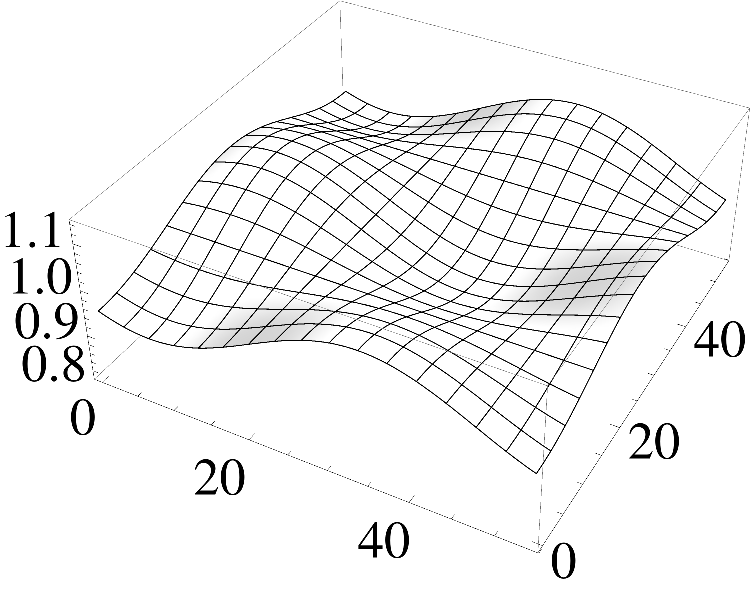
\includegraphics[width=0.45\linewidth]{Fig1}\label{fig:1a}} 
    \subfloat[]{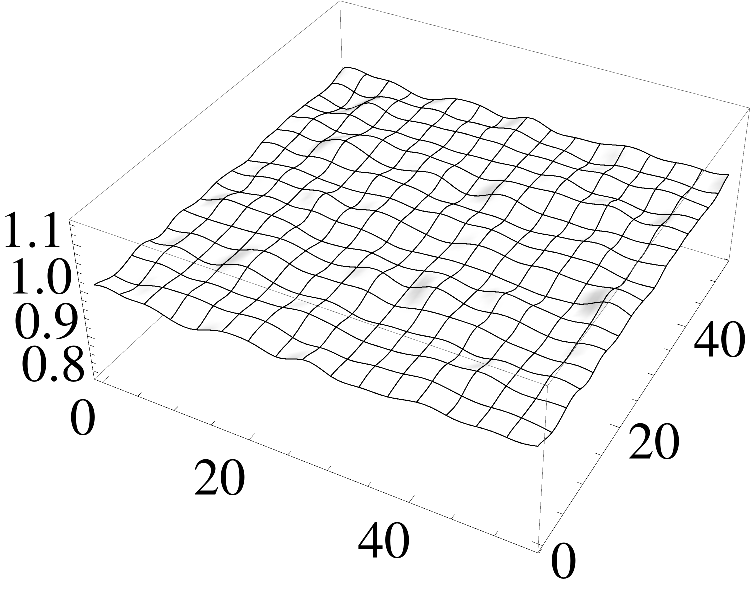
\includegraphics[width=0.45\linewidth]{Fig9}\label{fig:1b}} \\
    \subfloat[]{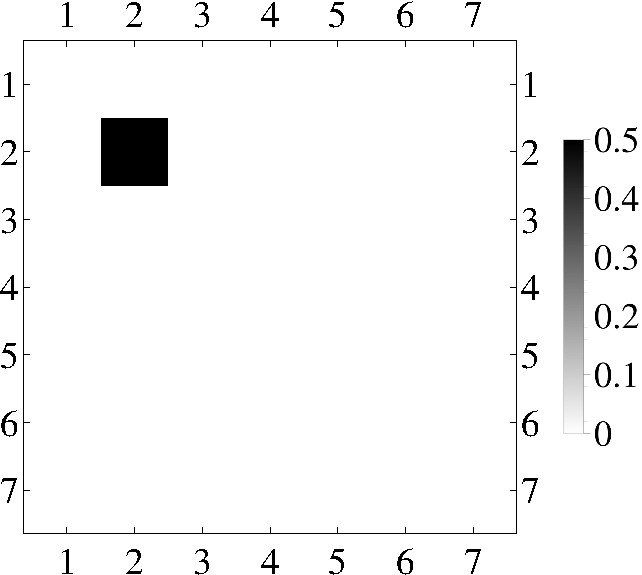
\includegraphics[width=0.45\linewidth]{Fig3}\label{fig:1c}}
    \subfloat[]{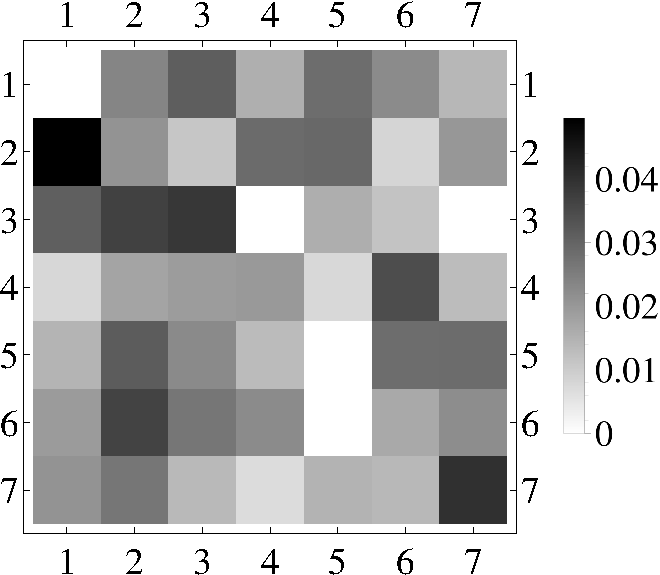
\includegraphics[width=0.45\linewidth]{Fig11}\label{fig:1d}}
   \caption{Two different initial conditions and their discrete Fourier transform frequency distributions. In \ref{fig_ic}\subref{fig:1a} a cosine initial condition $1 - 0.05 \left[ \cos [2 \pi x/L] + \sin [2 \pi x/]\right] \cos[2 \pi y/L]$ is used to excite a quiescent film. In \ref{fig_ic} \subref{fig:1a} a uniform random perturbation is used to excite the quiescent film.}
   \label{fig_ic}
  \end{figure}


%Effect of initial conditions on square domain
  \begin{figure} 
   \centering
    \subfloat[]{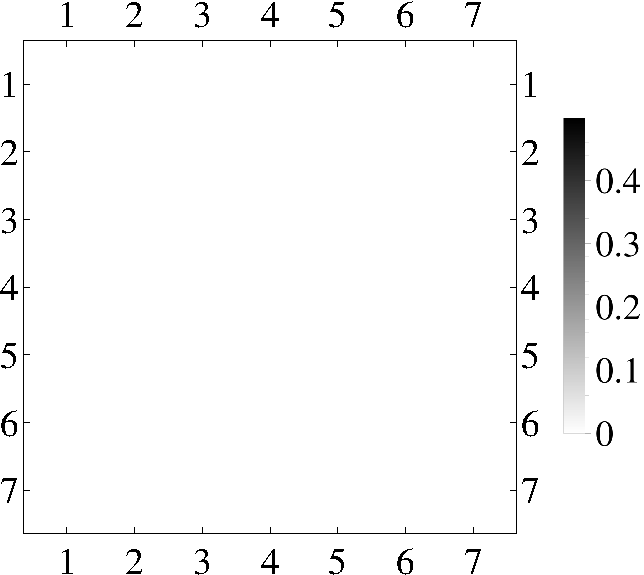
\includegraphics[width=0.45\linewidth]{Fig8}\label{fig:2a}} 
    \subfloat[]{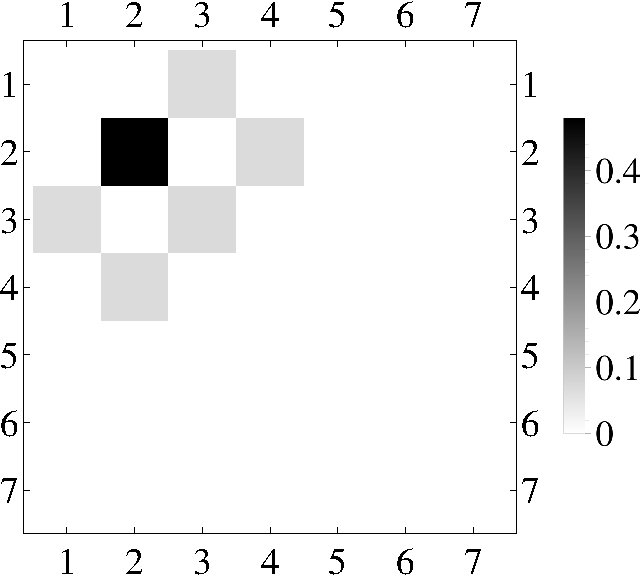
\includegraphics[width=0.45\linewidth]{Fig4}\label{fig:2b}}
%    \subfloat{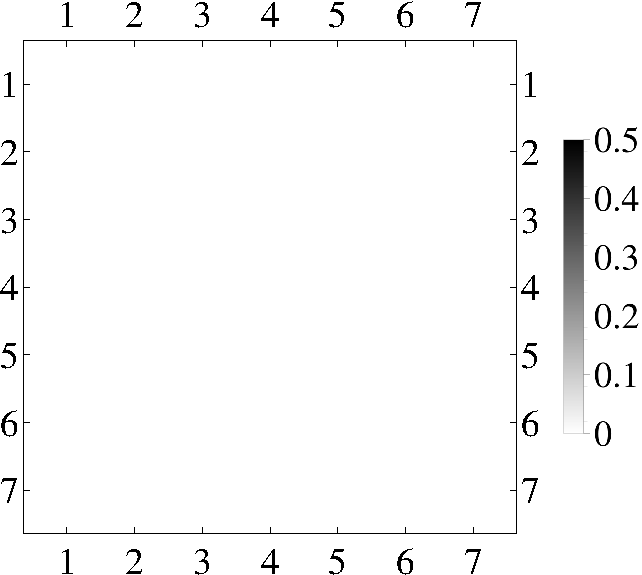
\includegraphics[width=0.4\linewidth]{Fig7}\label{fig:2d}}
   \caption{The effect of gravity on film dynamics for a square domain with $L=\lambda_\text{max}$. In \ref{fig_ic_effect}\subref{fig:2b}The discrete Fourier transforms show a cascade of frequencies for zero gravity. The dominant mode is that of the fastest growing wavelength.}
   \label{fig_ic_effect}
  \end{figure}


%Changing the domain size: Square/non-whole number and Rectangular/non-whole number
  \begin{figure} 
   \centering
    \subfloat[]{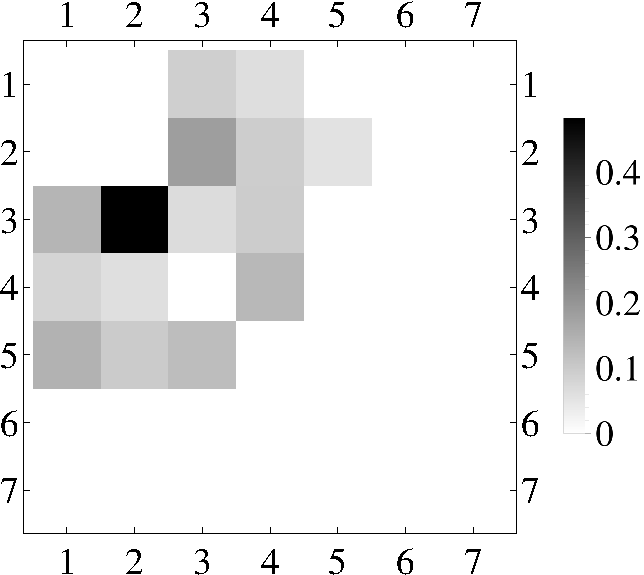
\includegraphics[width=0.45\linewidth]{Fig16}\label{fig:3a}} 
    \subfloat[]{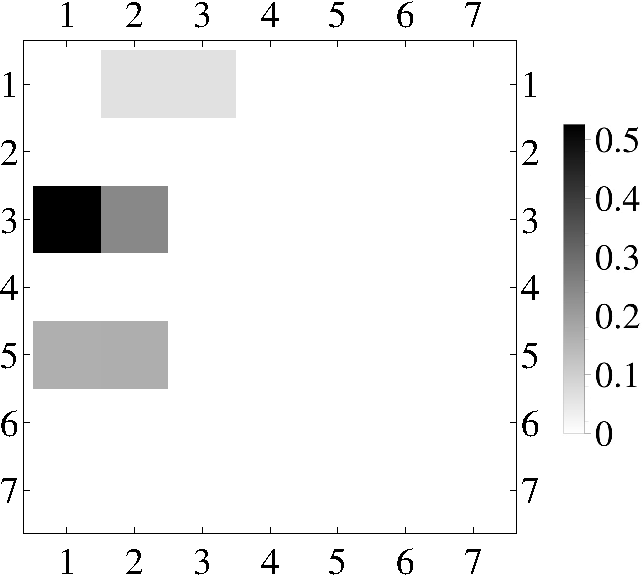
\includegraphics[width=0.45\linewidth]{Fig24}\label{fig:3b}} 
%    \subfloat{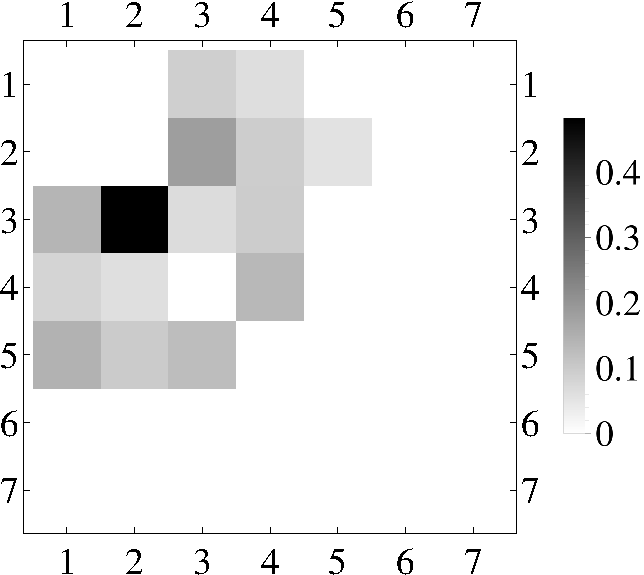
\includegraphics[width=0.45\linewidth]{Fig16}\label{fig:3c}}
%    \subfloat{\includegraphics[width=0.4\linewidth]{Fig20}\label{fig:3d}}
   \caption{The effect of domain size is shown with the cosine initial condition. A square domain is used with $L=2.238\lambda_\text{max}$ in figure \ref{fig_domain_size_effect} \subref{fig:3a} and a rectangular domain is used with $L_x = 2.238 \lambda_\text{max}, L_y=1.641 \lambda_\text{max}$ in figure \ref{fig_domain_size_effect} \subref{fig:3b}. The discrete Fourier transforms show a cascade of frequencies. The dominant mode is that of the fastest growing wavelength.}
   \label{fig_domain_size_effect}
  \end{figure}



%  \begin{figure} 
%   \centering
%    \subfloat{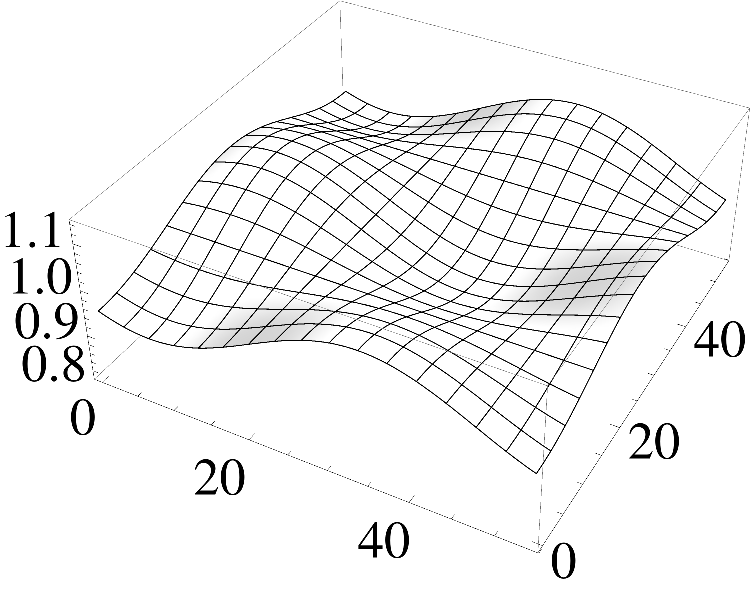
\includegraphics[width=0.45\linewidth]{Fig1}\label{fig:1a}} 
%    \subfloat{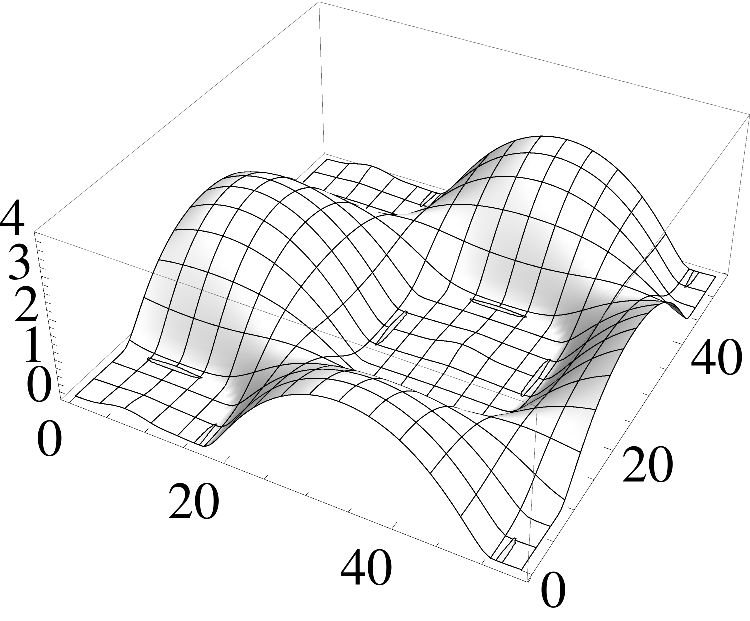
\includegraphics[width=0.45\linewidth]{Fig2}\label{fig:1b}} \\
%    \subfloat{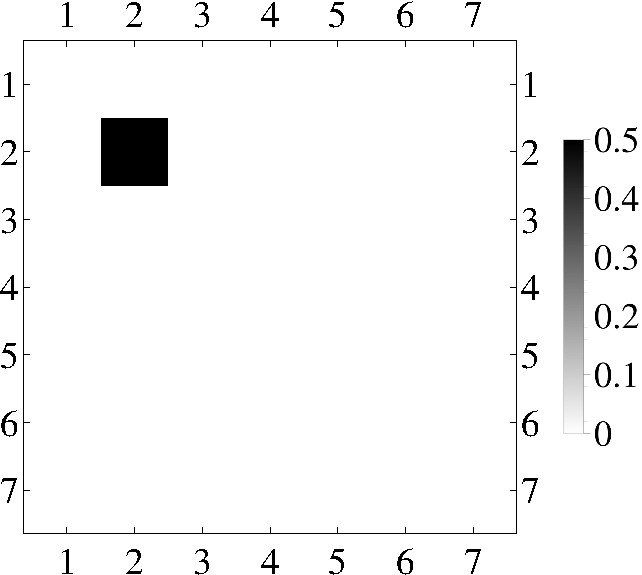
\includegraphics[width=0.45\linewidth]{Fig3}\label{fig:1c}}
%    \subfloat{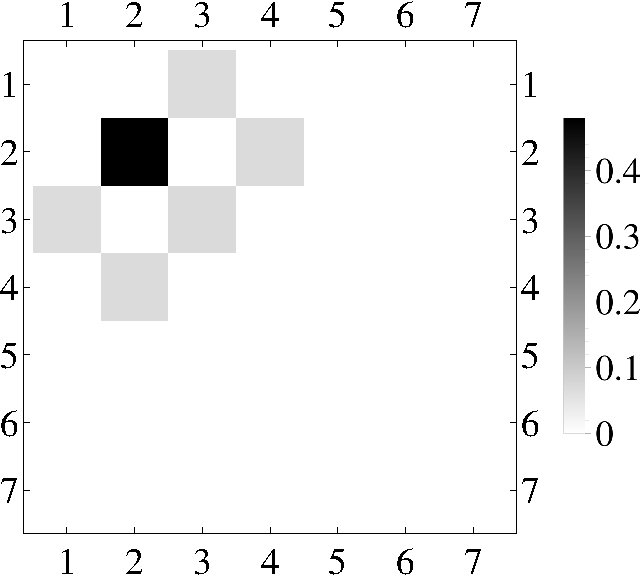
\includegraphics[width=0.4\linewidth]{Fig4}\label{fig:1d}}
%   \caption{2.35 millimeter DCM film evaporating in Earth's gravitational field. Film is depleted in 1 minute.}
%   \label{fig_eg}
%  \end{figure}



%  \begin{figure}
%   \centering
%    \subfloat{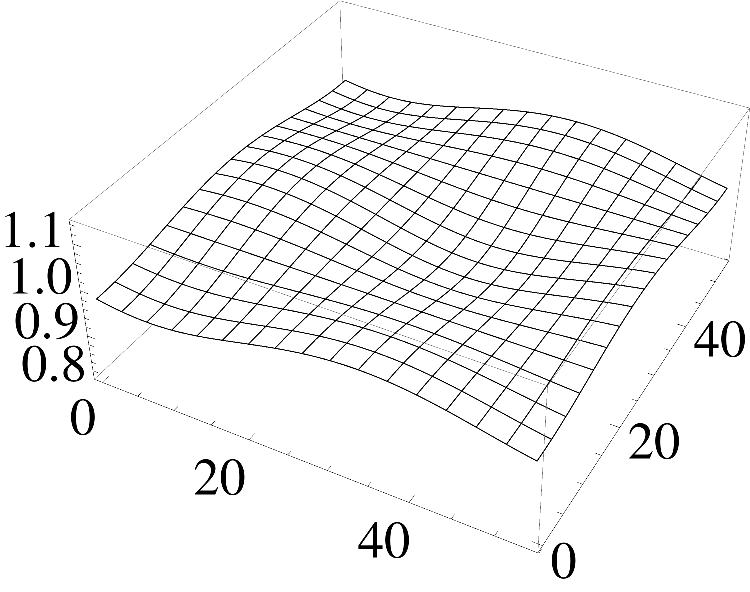
\includegraphics[width=0.45\linewidth]{Fig5}\label{fig:2a}}
%    \subfloat{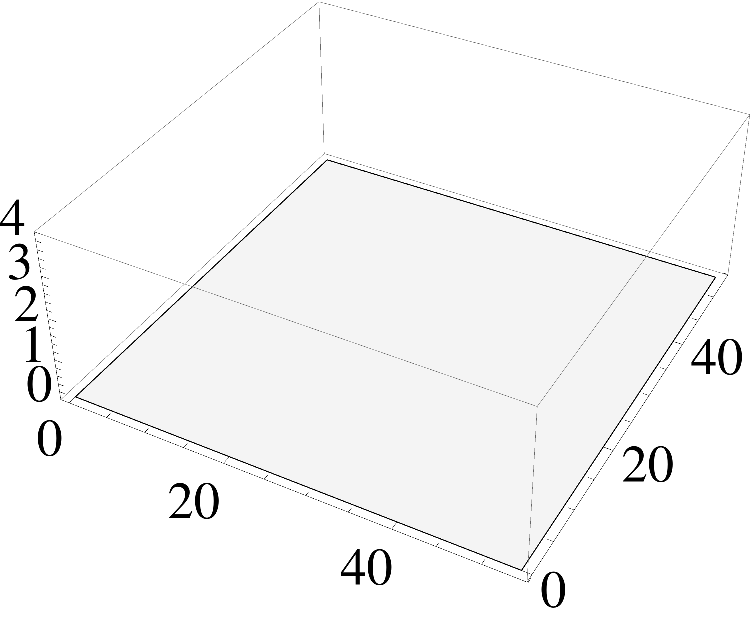
\includegraphics[width=0.45\linewidth]{Fig6}\label{fig:2b}} \\
%    \subfloat{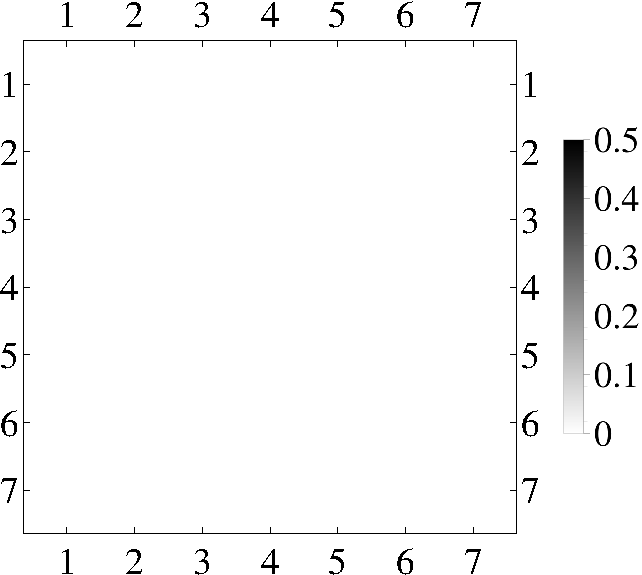
\includegraphics[width=0.45\linewidth]{Fig7}\label{fig:2c}}
%    \subfloat{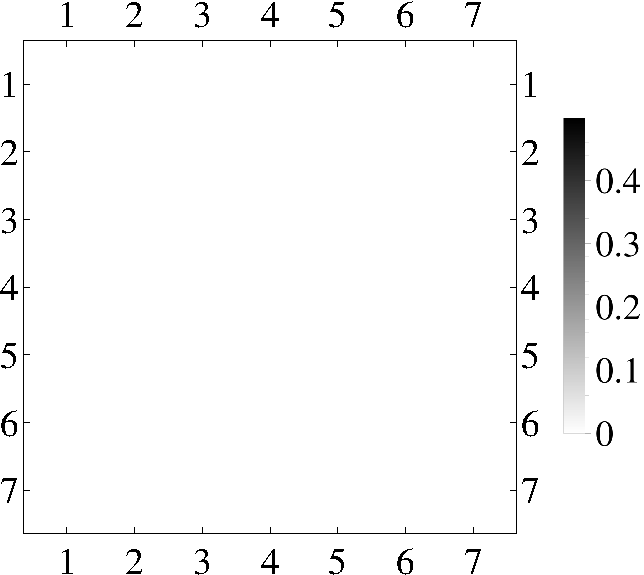
\includegraphics[width=0.45\linewidth]{Fig8}\label{fig:2d}}
%   \caption{2.35 millimeter DCM film evaporating in zero gravity. Film ruptures in 4 seconds. Thermocapillary fingers/long wave structures appear at rupture.}
%   \label{fig_zg}
%  \end{figure}

% \clearpage

%  \begin{figure}
%   \centering
%    \subfloat{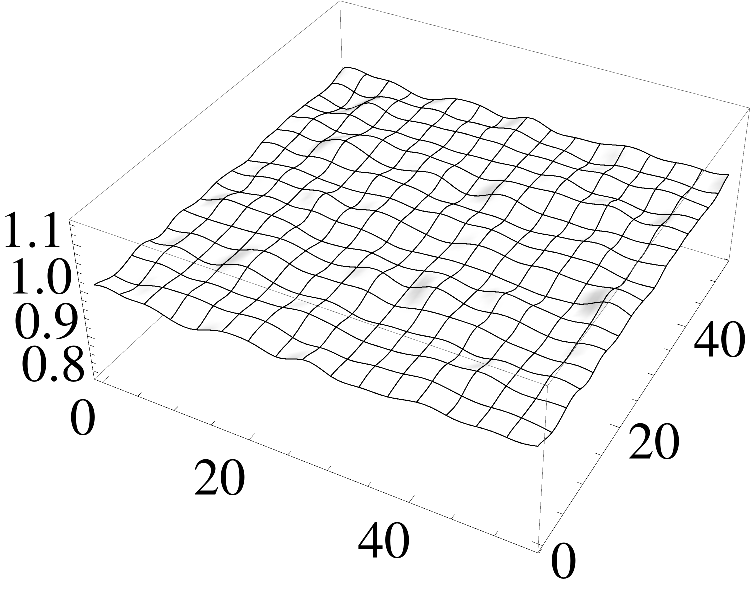
\includegraphics[width=0.45\linewidth]{Fig9}\label{fig:3aw}}
%    \subfloat{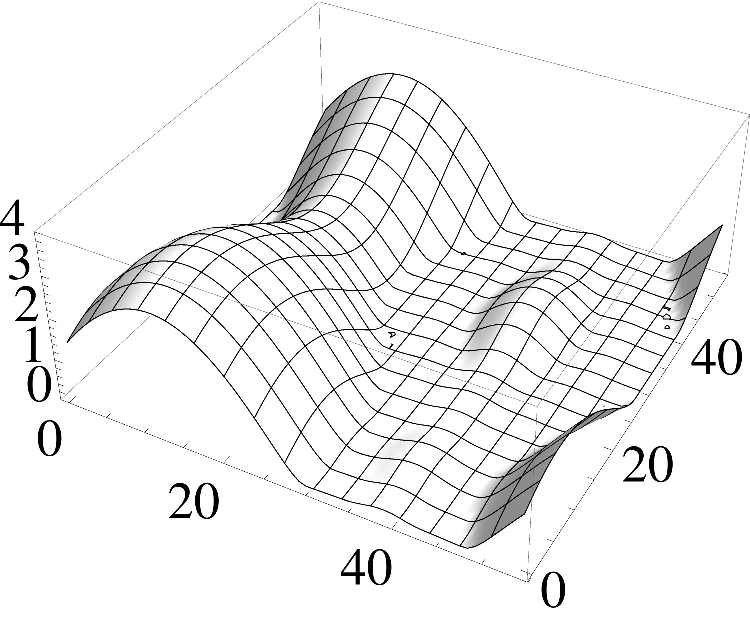
\includegraphics[width=0.45\linewidth]{Fig10}\label{fig:3bw}} \\
%    \subfloat{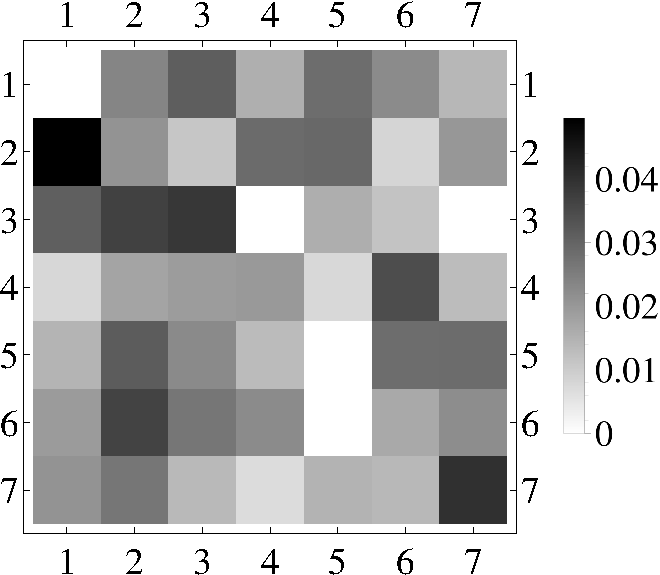
\includegraphics[width=0.45\linewidth]{Fig11}\label{fig:3cw}}
%    \subfloat{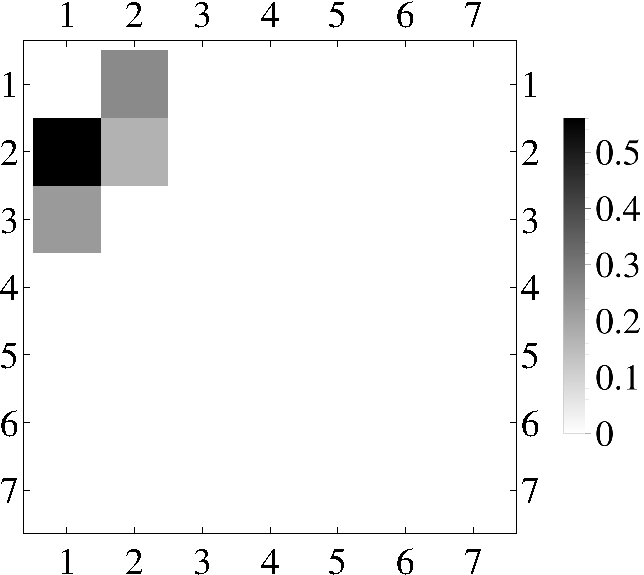
\includegraphics[width=0.45\linewidth]{Fig12}\label{fig:3dw}}
%   \caption{2.35 millimeter DCM film evaporating in zero gravity. Film ruptures in 4 seconds. Uniform random initial condition is applie. The domain is square with it's side length, $L=\lambda_\text{max}$. Thermocapillary fingers/long wave structures appear at rupture.}
%   \label{random_1_whole}
%  \end{figure}




% \clearpage


%  \begin{figure} 
%   \centering
%    \subfloat{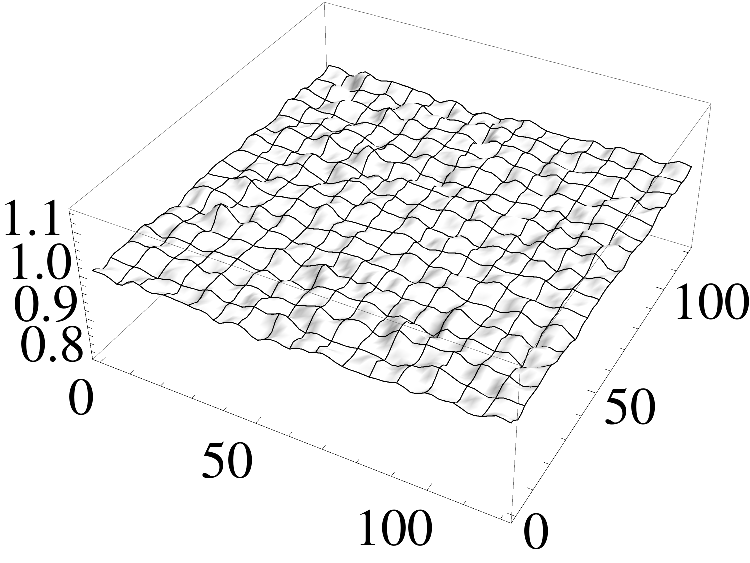
\includegraphics[width=0.45\linewidth]{Fig13}\label{fig:3a}} 
%    \subfloat{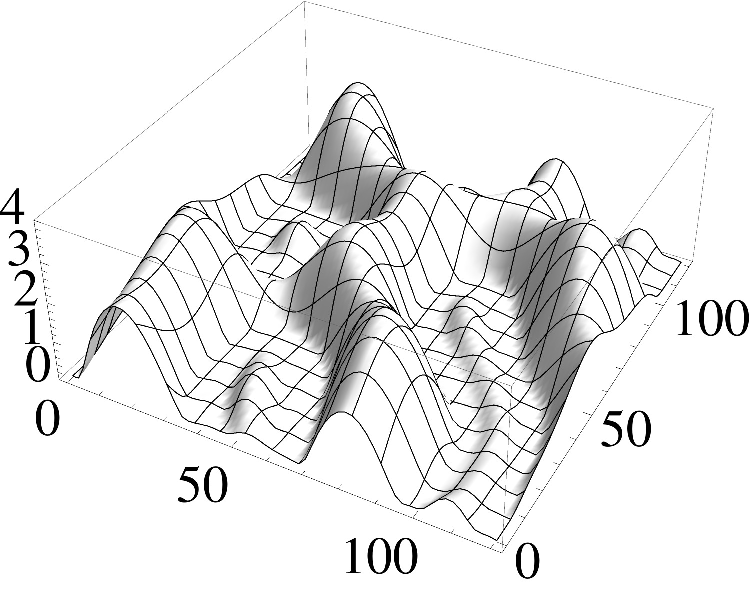
\includegraphics[width=0.45\linewidth]{Fig14}\label{fig:3b}} \\
%    \subfloat{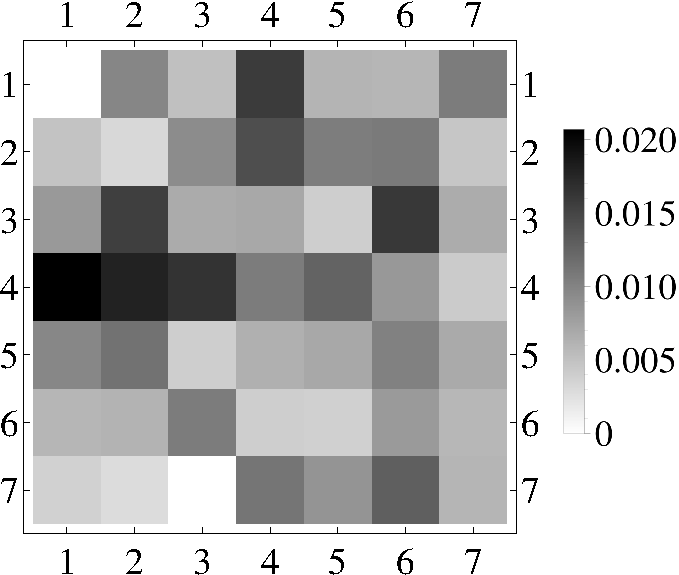
\includegraphics[width=0.45\linewidth]{Fig15}\label{fig:3c}}
%    \subfloat{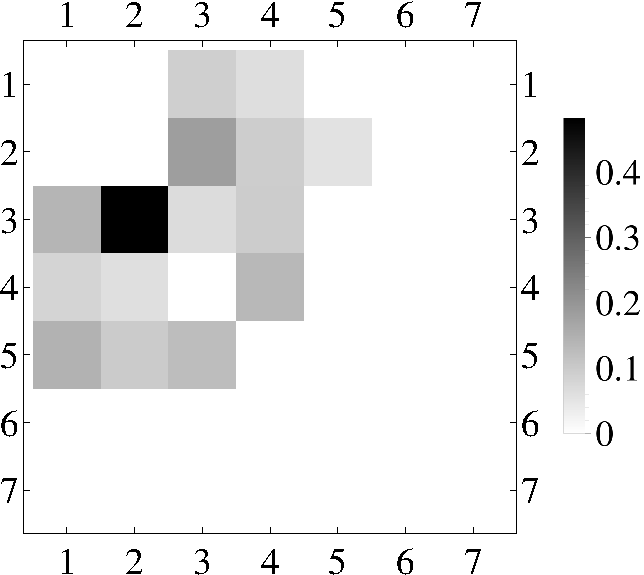
\includegraphics[width=0.45\linewidth]{Fig16}\label{fig:3d}}
%   \caption{2.35 millimeter DCM film evaporating in zero gravity, subject to a uniform random initial condition. The domain size is square with it's side-length equal to $L = 2.238 \lambda_\text{max}$. Film ruptures in about 4 seconds. The fastest growing wavelength appears as dominant mode at rupture.}
%   \label{random_1}  \end{figure}



%  \begin{figure}
%   \centering
%    \subfloat{\includegraphics[width=0.45\linewidth]{Fig17}\label{fig:3ar}}
%    \subfloat{\includegraphics[width=0.45\linewidth]{Fig18}\label{fig:3br}} \\
%    \subfloat{\includegraphics[width=0.45\linewidth]{Fig19}\label{fig:3cr}}
%    \subfloat{\includegraphics[width=0.45\linewidth]{Fig20}\label{fig:3dr}}
%   \caption{2.35 millimeter DCM film evaporating in zero gravity, subject to a uniform random initial condition. The domain size is square with it's side-length equal to $L = 2.238 \lambda_\text{max}$. Film ruptures in about 4 seconds. The fastest growing wavelength appears as dominant mode at rupture.}
%   \label{random_1_repeat}  \end{figure}




%  \begin{figure} 
%   \centering
%    \subfloat{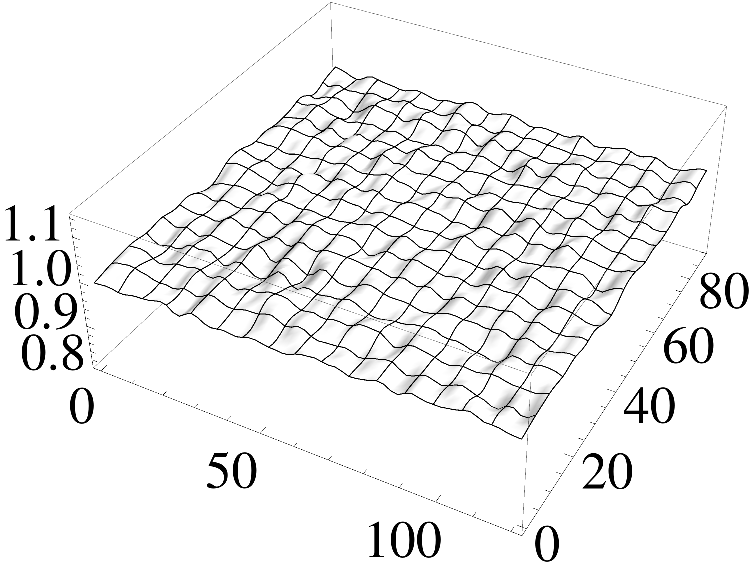
\includegraphics[width=0.45\linewidth]{Fig21}\label{fig:4a}} 
%    \subfloat{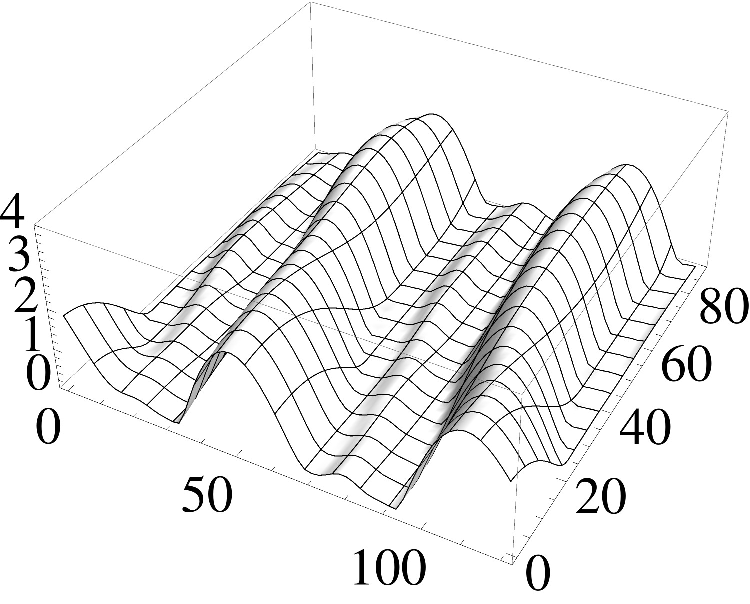
\includegraphics[width=0.45\linewidth]{Fig22}\label{fig:4b}} \\
%    \subfloat{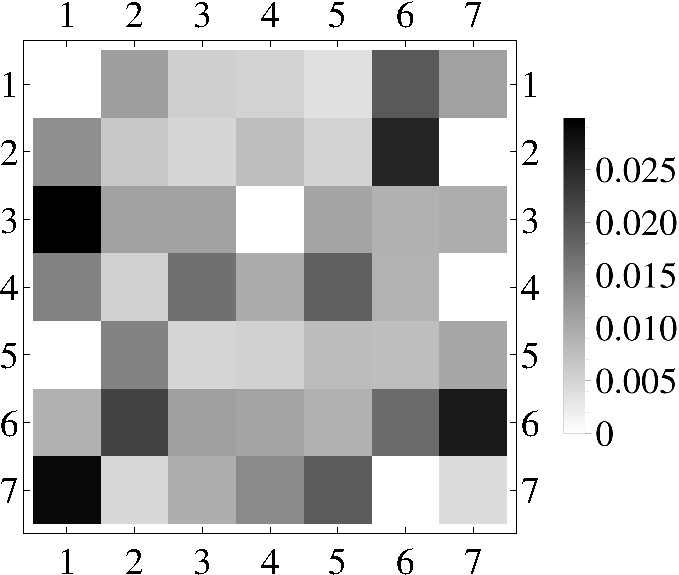
\includegraphics[width=0.45\linewidth]{Fig23}\label{fig:4c}}
%    \subfloat{\includegraphics[width=0.45\linewidth]{Fig24}\label{fig:4d}}
%   \caption{Evaporating Dichloromethane (DCM) film evolving after a uniform random initial condition is imposed in zero gravity. The initial film thickness is $2.35 mm$. The domain is rectangular with length and breadth respectively equal to $2.238 \lambda_\text{max}$ and $1.641 \lambda_\text{max}$. Cascade of superharmonics appears in the longer dimension. The fastest growing wavelength holds most of the energy at rupture. Film ruptures in 4 seconds.}
%   \label{rndm2}
%  \end{figure}


% \clearpage

  \begin{figure}
   \centering
   \includegraphics[width=\linewidth]{Fig25} 	
   \caption{The growth rate of long wave instabilities for varying film thickness ($h=0.2$ to $1.0$) for a $2.35$ mm film evaporating in zero gravity ($Bo=0.0$). As the film thickness decreases, the range of perturbation wavenumbers for which long wave instabilities set in increases. Film thickness is scaled with $h_0=2.35$mm.}
   \label{omega_q_1}
  \end{figure}

% \clearpage


  \begin{figure}
   \centering
   \includegraphics[width=\linewidth]{Fig26}
   \caption{The growth rate of long wave instabilities for varying film thickness for a $2.35$ mm film evaporating in micro-gravity ($Bo=0.01$). As the film thickness decreases, the range of perturbation wavenumbers for which long wave instabilities set in increases. However, as a result of some gravity stabilization, the growth rate of long wave instabilities is lower than in the zero gravity case in figure \ref{omega_q_1}.Film thickness is scaled with $h_0=2.35$mm.}
   \label{omega_q_2}
  \end{figure}


  \begin{figure}
   \centering
   \includegraphics[width=\linewidth]{Fig27_2}
   \caption{Film thickness is plotted for $\omega=0$ (solid) and $\omega=-0.0004$ (dashed) for different perturbation wavenumbers, q.This plot allows for the identification of the thickness of DCM film that is stable to long wave modes.}
   \label{h_vs_q}
  \end{figure}

\end{document}
